
Previously,\footnote{See Part II, section 5} we learned how to write handwritten code in an implementation file, then generate
a \emph{partial class} to inject code into the metamodel. Now however, we'll generate and edit a partial class to automaticall insert code into the
corresponding Java file, which will then inject into the metamodel.

\begin{itemize}

\item[$\blacktriangleright$] Go to ``BoxImpl.java'' and, without editing any method signatures there, generate its corresponding injection file by either right
clicking the file in the package explorer or within the editor window (Fig.~\ref{}).

\item[$\blacktriangleright$] A second file should now be placed in the \texttt{injection} folder. Open \texttt{BomxImple.inject} and notice the
partial class includes every method declaration but (as expected) no implementation code (Fig.~\ref{fig:injection_partialClassBox}).

\begin{figure}[htbp]
    \centering
    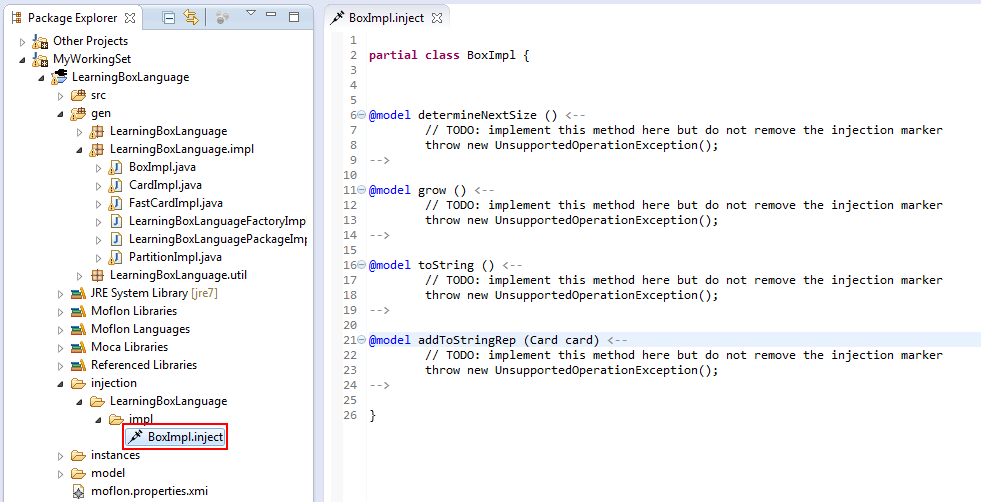
\includegraphics[width=1.0\textwidth]{eclipse_injectionBoxImpl}
    \caption{Generated Injection file for \texttt{BoxImpl.java}}
    \label{fig:injection_partialClassBox}
\end{figure}

\item[$\blacktriangleright$] Complete the \texttt{addToStringRep} and \texttt{determineNextSize} methods as specified in Fig.~\ref{code:complete_inject_file}
below.

\vspace{0.5cm}

\begin{figure}[htbp]
        \centering
        \begin{lstlisting}[language=Java, keywordstyle={\bfseries\color{purple}}, backgroundcolor=\color{white}]
    @model addToStringRep (Card card) <--

            StringBuilder sb = new StringBuilder();

            if (stringRep == null)
            {
                sb.append("BoxContent: [");

            }
            else
            {
                sb.append(stringRep);
                sb.append(", [");
            }

            sb.append(card.getFace());
            sb.append(", ");
            sb.append(card.getBack());
            sb.append("]");

            stringRep = sb.toString();
    -->

    @model determineNextSize () <--

            return getContainedPartition().size() * 10;
    -->

        \end{lstlisting}
        \caption{Implementation of helper methods as an injection}
        \label{code:complete_inject_file}
    \end{figure}
    \FloatBarrier

\vspace{0.5cm}

\item[$\blacktriangleright$] Right-click the injection file, and rebuild your project by selecting ``eMoflon/Clean and
Build''(Fig~\ref{fig:eclipse_buildFromInjecton}).

\item[$\blacktriangleright$] The helper methods should now be implemented in \texttt{BoxImpl.java}, which can be found under
the ``/gen/LearningBoxLanguage.impl'' package (Fig~\ref{fig:eclipse_updatedBoxImpl}).

\item[$\blacktriangleright$] For additional information on injections, check out Part IV: Miscellaneous.\footnote{Download link: \dlPartSix}. Be sure to also
review the work we completed with injections in Part II: Ecore.\footnote{Download Link: \dlPartTwo}

\newpage

\vspace*{2cm}

\begin{figure}[htbp]
    \centering
    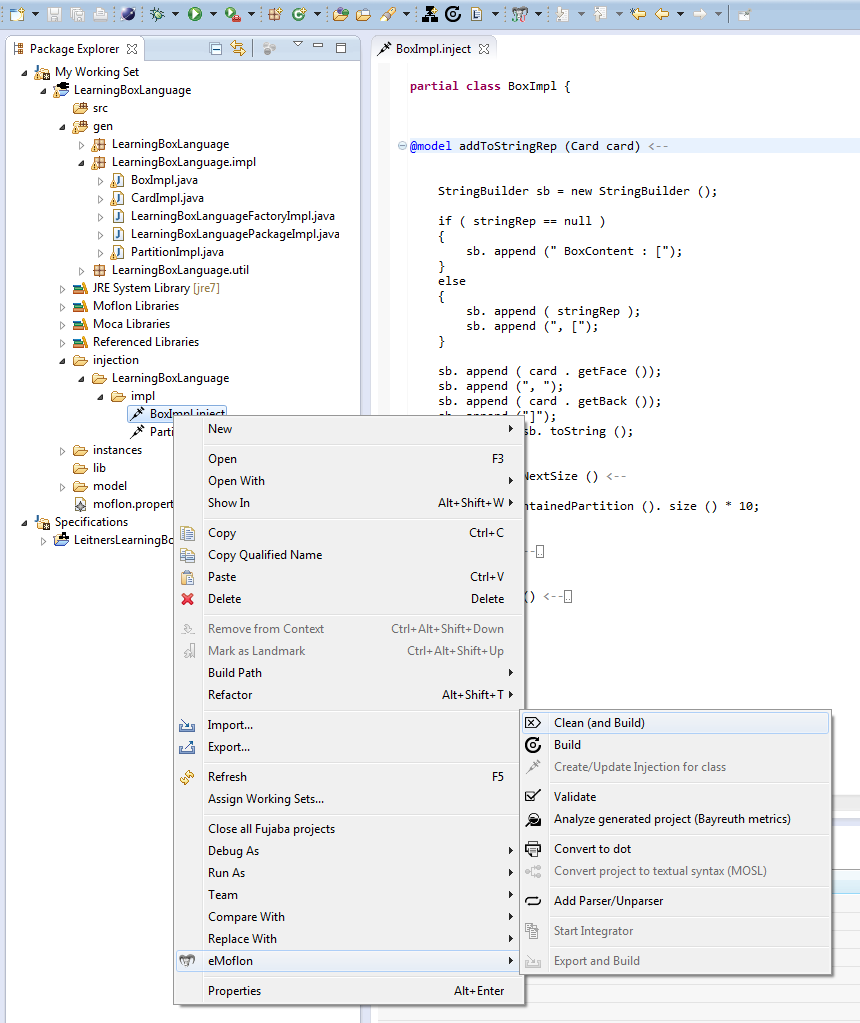
\includegraphics[width=\textwidth]{eclipse_buildFromInject}
    \caption{Build the entire project from the injection file}
    \label{fig:eclipse_buildFromInjecton}
\end{figure}

\newpage

\vspace*{2cm}

\begin{figure}[htbp]
    \centering
    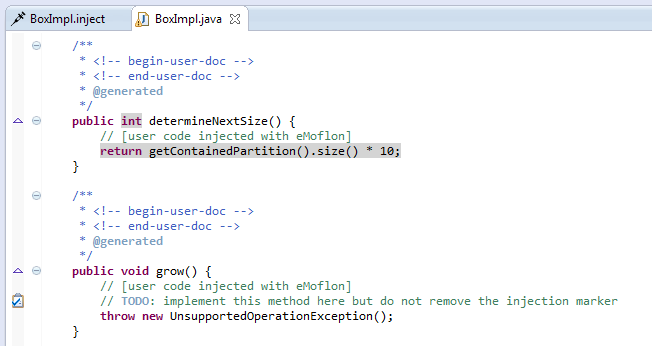
\includegraphics[width=\textwidth]{eclipse_updatedBoxImpl}
    \caption{Updated \texttt{BoxImpl.java} file}
    \label{fig:eclipse_updatedBoxImpl}
\end{figure}

\fancyfoot[R]{ $\triangleright$ \hyperlink{growBox vis}{Next [visual]\hspace{0.2cm} } \\ $\triangleright$ \hyperlink{growBox tex}{Next [textual]} }

\end{itemize}

